% % % % % % % % % % % % % % % % % % % % % % % % % % % % % % % % % % % % % % % % % % % %
%                                                                                     %
% Short Sectioned Assignment LaTeX Template Version 1.0 (5/5/12)                      %
% This template has been downloaded from: http://www.LaTeXTemplates.com               %
%                                                                                     %
% Original author:  Frits Wenneker (http://www.howtotex.com)                          %
%                                                                                     %
% Modified by: Fco Javier Sueza Rodríguez (fcosueza@disroot.org)                      %
%                                                                                     %
% Changes:                                                                            %
%	    - Custom Chapters, Sections and Subsections (titlesec package)                %
%           - Document type scrbook (oneside)                                         %
%           - Use babel-lang-spanish package and marvosym                             %
%           - Use hyperref, enumitem, tcolorbox and glossaries packages               %
%           - Use Time New Roman (mathptmx), Helvetic and Courier fonts               %
%                                                                                     %
% License: CC BY-NC-SA 3.0 (http://creativecommons.org/licenses/by-nc-sa/3.0/)        %
%                                                                                     %
% % % % % % % % % % % % % % % % % % % % % % % % % % % % % % % % % % % % % % % % % % % %

%-----------------------------------------------%
%	              Packages                  %
%-----------------------------------------------%

\documentclass[paper=a4, fontsize=11pt, oneside]{scrbook}

% ---- Text Input/Output ----- %

\usepackage[T1]{fontenc}
\usepackage[utf8]{inputenc}
\usepackage{mathptmx}
\usepackage[scaled=.92]{helvet}
\usepackage{courier}
\usepackage[indent=12pt]{parskip}

\usepackage{geometry}
\geometry{verbose,tmargin=3cm,bmargin=3cm,lmargin=2.6cm,rmargin=2.6cm}

% ---- Language ----- %

\usepackage[spanish]{babel}
\usepackage{marvosym}

% ---- Another packages ---- %

\usepackage{amsmath,amsfonts,amsthm}
\usepackage{graphics,graphicx}
\usepackage{titlesec}
\usepackage{fancyhdr}
\usepackage{tcolorbox}
\usepackage{hyperref}
\usepackage{enumitem}
\usepackage[automake]{glossaries}

%--------------------------------------------------------------------%
%                      Customizing Document                          %
%--------------------------------------------------------------------%


% ----------- Custom Chapters, Sections and Subsections -------------- %

\titleformat{\chapter}[display]
			{\bfseries\Huge}
			{Tema \ \thechapter} {0.5ex}
			{\vspace{1ex}\centering}

\titleformat{\section}[hang]
			{\bfseries\Large}
			{\thesection}{0.5em}{}

\titleformat{\subsection}[hang]
			{\bfseries\large}
			{\thesubsection}{0.5em}{}

\titleformat{\subsubsection}[hang]
			{\bfseries\large}
			{\thesubsubsection}{0.5em}{}

\hypersetup{
    colorlinks=true,
    linkcolor=black,
    urlcolor=magenta
}

% ------------------- Custom heaaders and footers ------------------- %

\pagestyle{fancyplain}

\fancyhead[]{}
\fancyfoot[L]{}
\fancyfoot[C]{}
\fancyfoot[R]{\thepage}

\renewcommand{\headrulewidth}{0pt} % Remove header underlines
\renewcommand{\footrulewidth}{0pt} % Remove footer underlines

\setlength{\headheight}{13.6pt} % Customize the height of the header

% --------- Numbering equations, figures and tables ----------------- %

\numberwithin{equation}{section} % Number equations within sections
\numberwithin{figure}{section} % Number figures within sections
\numberwithin{table}{section} % Number tables within sections

% ------------------------ New Commands ----------------------------- %

\newcommand{\horrule}[1]{\rule{\linewidth}{#1}} % Create horizontal rule command


%----------------------------------------------------------------------------------------
%	TÍTULO Y DATOS DEL ALUMNO
%----------------------------------------------------------------------------------------

\title{
\vspace{10ex}
\normalfont \normalsize
\huge \textbf{Tarea 3: Introducción a la Gestión Empresarial de RRSS}
}
\author{Francisco Javier Sueza Rodríguez}
\date{\normalsize\today}

%----------------------------------------------------------------------------------------
%                                     DOCUMENTO
%----------------------------------------------------------------------------------------
\begin{document}

\maketitle

\thispagestyle{empty}

\vspace{65ex}

\begin{center}
    \begin{tabular}{l l}
        \textbf{Centro}: & IES Aguadulce \\
        \textbf{Ciclo Formativo}: & Desarrollo Aplicaciones Web (Distancia)\\
        \textbf{Asignatura}: & Horas de Libre Configuración\\
        \textbf{Tema}: & Tema 3 - Introducción a la Gestión Empresarial de RRSS\\
    \end{tabular}
\end{center}

\newpage

\tableofcontents

\vspace{30ex}

\listoffigures

\newpage

\section{Introducción}
Actualmente la mayoría de ofertas de trabajo y consultoras revisan los perfiles de linkedin para buscar a sus candidatos, el típico CV en papel ya no se utiliza. Así que vamos a ponernos manos a la obra y a crear un buen perfil de linkedin para que se fijen en nosotros.

\section{Ejercicio 1: Creando mi perfil de Linkedin}
\subsection{Enunciado}
\begin{enumerate}
    \item Si no tienes cuenta creada en Linkedin, crea una, rellenando todos los campos: extracto, experiencia, aptitudes, cursos. Busca contactos.
    \item Inserta tu foto de perfil. Recuerda que esta debe ser adecuada para este tipo de red profesional.
    \item Inserta la imagen del fondo de la cabecera. Pon una foto auténtica y hecha por ti, que identifique un poco tus intereses profesionales ( puedes buscar perfiles parecidos al tuyo a ver que tienen puesto para coger ideas).
    \item Añade la sección Acerca de .. y defínete en 5 líneas a nivel profesional y algo personal. Intenta utilizar sustantivos para empezar las frases, del tipo: creativo, sociable con capacidad para el trabajo en equipo... Añade 5 actitudes.
    \item Revisa el perfil de cinco contactos como mínimo que consideres que pueden adaptarse o servirte por ser afín a tu perfil.
    \item Prueba la búsqueda avanzada: busca contactos, empresas y grupos de un sector o varios sectores que te interesen.
    \item Haz una búsqueda de empleo e incluye la captura de la búsqueda en el documento.
    \item Comparte tu url de LinkedIn en el hilo del foro de la unidad: URL LinkedIn.
\end{enumerate}

\subsection{Solución}
En este ejercicio vamos a crear un perfil de Linkedin. En mi caso, ya lo tengo creado por lo que solo vamos a completar los apartados que aún no tengo completos.

\begin{enumerate}
    \item Este primer paso no ha sido necesario, ya que tengo una cuenta de Linkedin desde unos cuantos años. En la siguiente imagen se puede ver una captura de la cuenta.

    \begin{figure}[H]
        \centering
        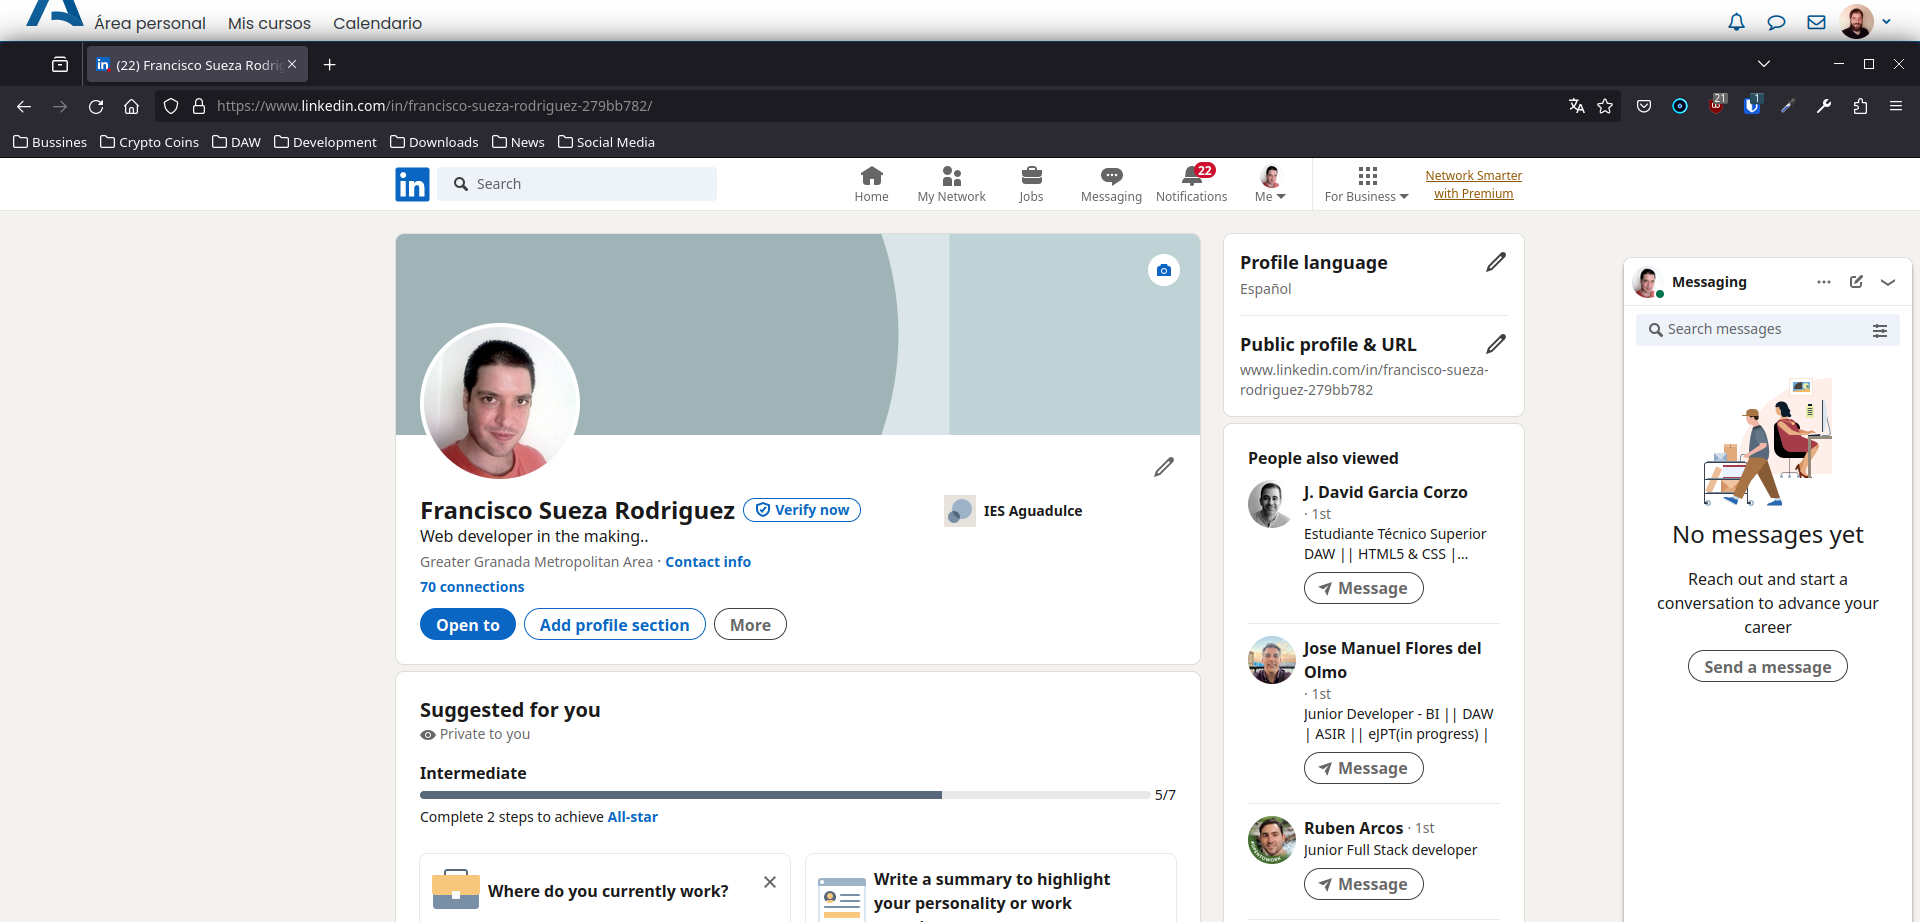
\includegraphics[scale=0.20]{perfil-link.png}
        \caption{Perfil de Linkedin}
    \end{figure}

    \item Una vez creado nuestro perfil, para añadir una foto pulsamos sobre  la foto que hay encima del nombre en el perfil y se nos mostrará una ventana con la opción \textit{Add photo}, donde podremos seleccionar la foto que queremos subir a nuestro perfil, como se ve en la siguiente captura.

    \begin{figure}[H]
        \centering
        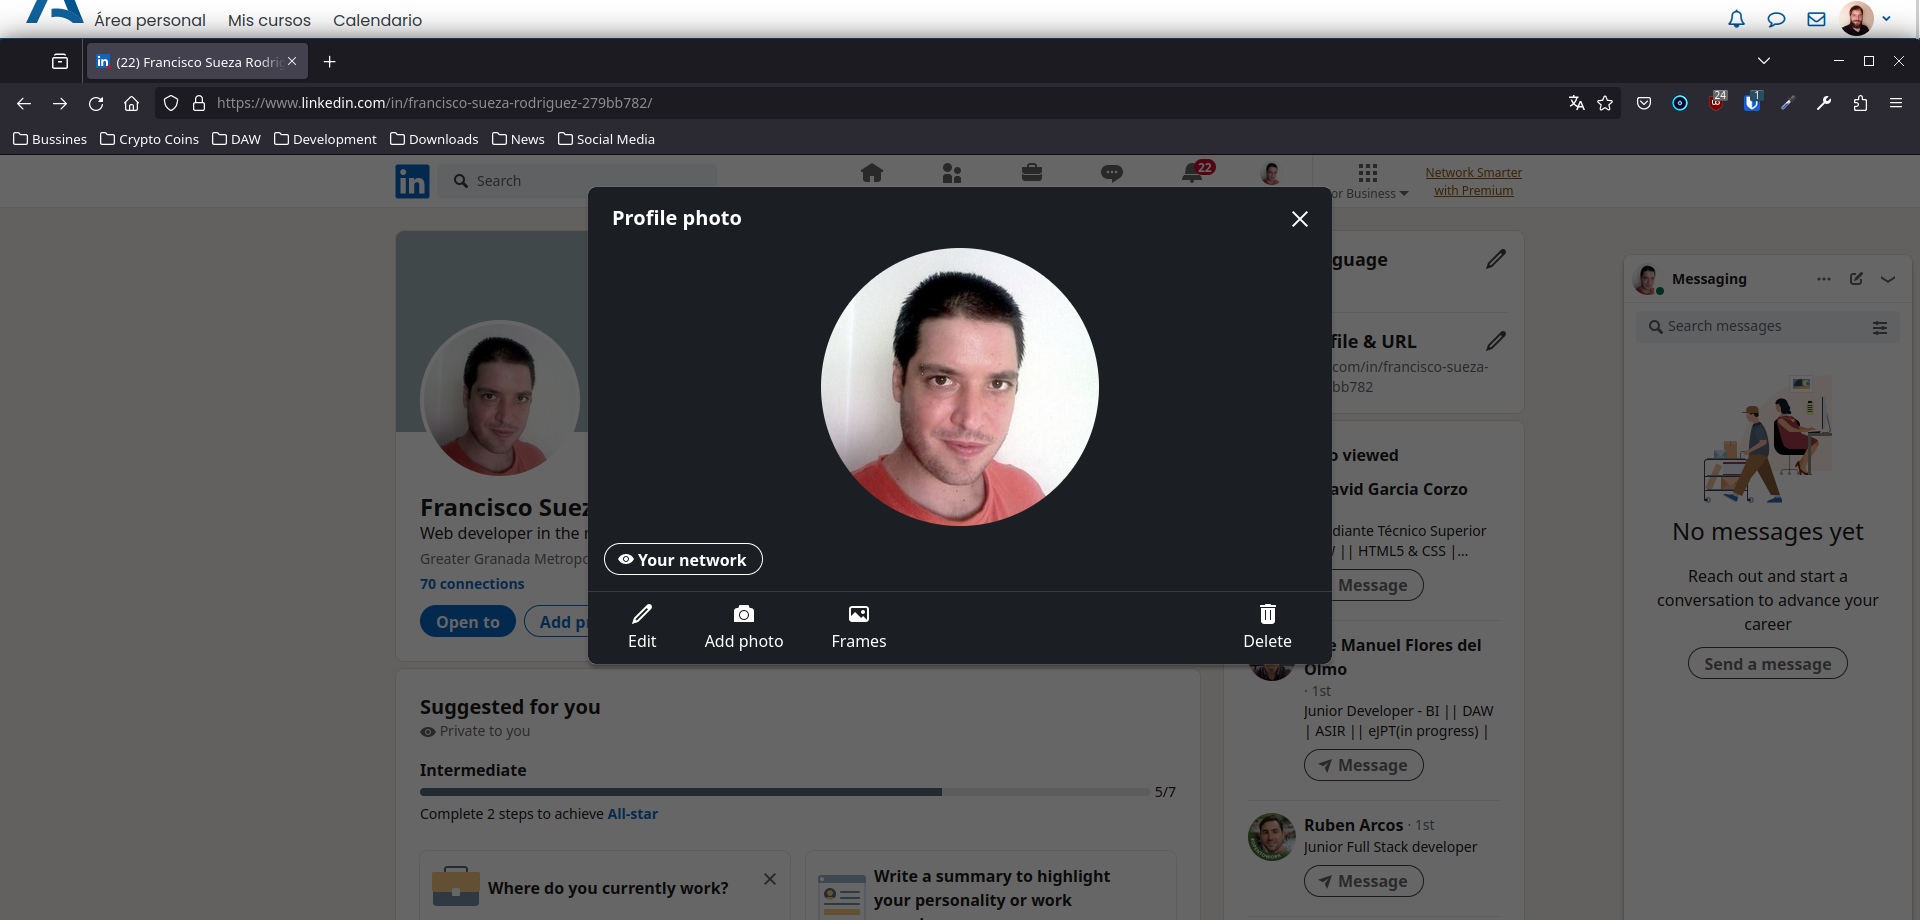
\includegraphics[scale=0.27]{perfil-link-foto.png}
        \caption{Añadiendo la foto al perfil}
    \end{figure}

    \item El siguiente paso es añadir la imagen de portada. Para ello, pulsamos en el icono de una cámara de fotos, que podemos ver en la esquina superior derecha de la imagen de portada, que nos abrirá una ventana donde podremos seleccionar la imagen que queremos como fondo.

    \begin{figure}[H]
        \centering
        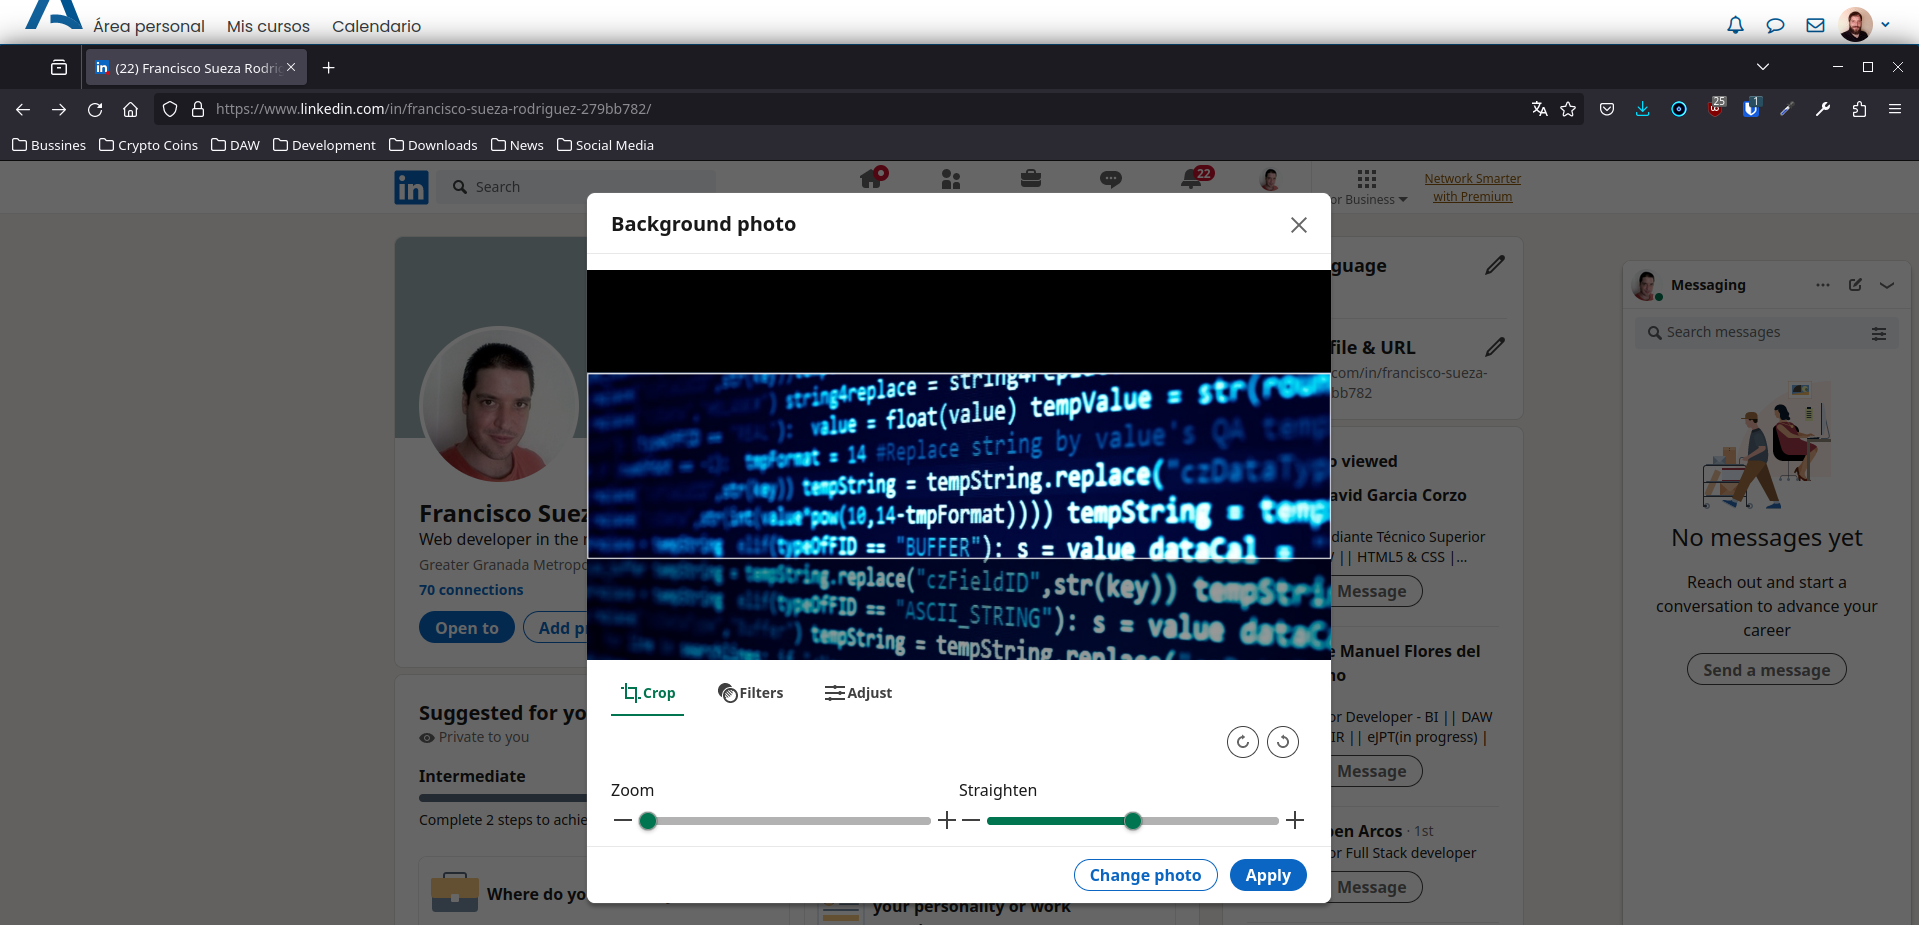
\includegraphics[scale=0.27]{perfil-link-back.png}
        \caption{Selección de la imagen de fondo}
    \end{figure}

    \item En este paso baso a añadir la sección \textit{Acerca de}. Para ello, debemos pulsar en el botón \textit{Add profile section} y dentro del menú que se nos mostrará en la opción \textit{Add About}. Una vez aquí, se nos mostrará una formulario donde podremos introducir la información sobre nosotros que creamos relevante para nuestro perfil, como podemos ver en la siguiente figura.

    \begin{figure}[H]
        \centering
        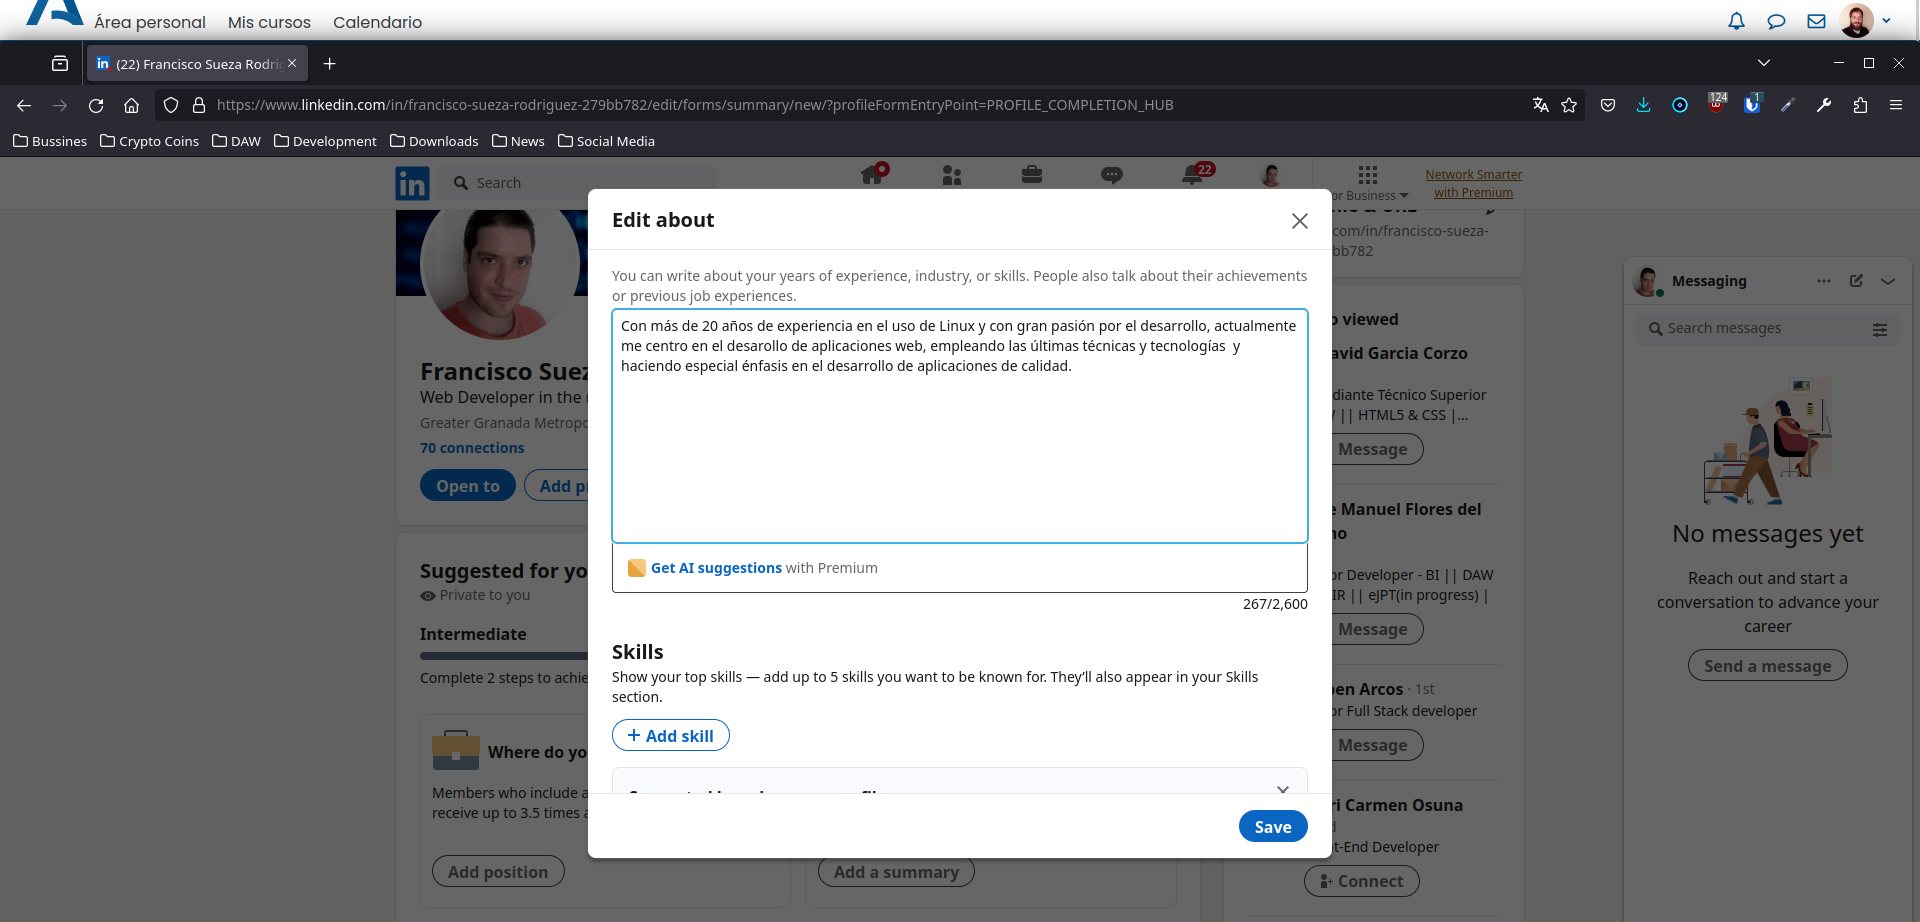
\includegraphics[scale=0.25]{perfil-link-about.png}
        \caption{Añadiendo sección Acerca de}
    \end{figure}

    \item En este punto se han visitado 5 perfiles que usuario que pueden ser relevantes en nuestra búsqueda de empleo. Por motivos de privacidad, no se van a incluir capturas de la visita de estos perfiles, sino que se van a incluir un lista de enlaces a dichos perfiles. Para visitar los perfiles de nuestro contactos, debemos pulsar en el enlace \textit{conecctions} que aparece debajo de nuestra foto de perfil, donde se mostrarán nuestros contactos.

    \begin{itemize}
        \item \url{https://www.linkedin.com/in/mcosuna/}
        \item \url{https://www.linkedin.com/in/josecegra/}
        \item \url{https://www.linkedin.com/in/opsidao/}
        \item \url{https://www.linkedin.com/in/nazariogarcia/}
        \item \url{https://www.linkedin.com/in/victor-m-espinosa-2380356a/}
    \end{itemize}

    \item A continuación, hemos realizado una búsqueda. Para ello, hemos introducido el término que queríamos buscar en la casilla de búsqueda que encontramos arriba a la izquierda. En nuestro caso, el termino ha sido \textit{Javascript}, para encontrar grupos relacionados con este lenguaje de programación, como podemos ver en la siguiente captura. Podemos ver el resultado a continuación.

        \begin{figure}[H]
        \centering
        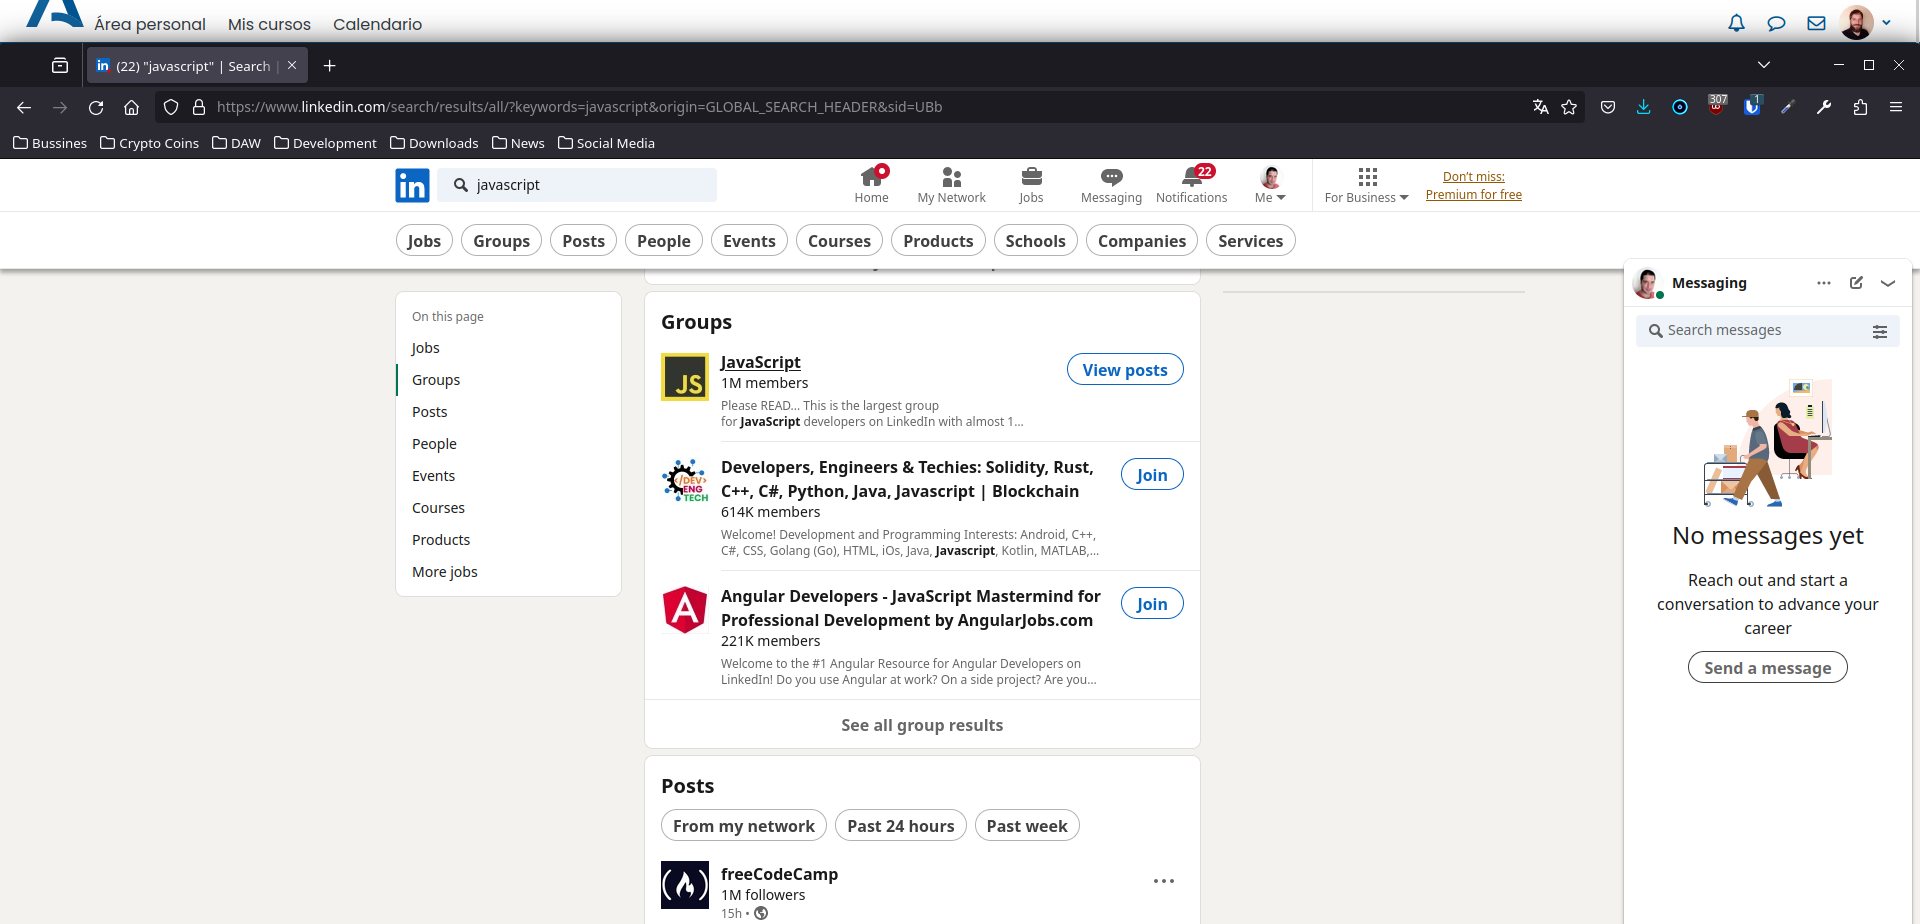
\includegraphics[scale=0.25]{perfil-link-search.png}
        \caption{Realizando una búsqueda}
    \end{figure}

    \item La siguiente búsqueda que se ha realizado ha sido la de empleos.  Para ello, pulsamos en la pestaña \textit{Jobs} que podemos encontrar en la parte superior del perfil. Una vez pulsada, nos mostrará la casilla de búsqueda, donde podremos realizar un búsqueda por habilidades, puestos,..etc. Además nos mostrará varios tags con opciones de búsqueda acordes a nuestro perfil. He pulsado en \textit{Junior Web Developer} y el resultado de la búsqueda es el siguiente.

    \begin{figure}[H]
        \centering
        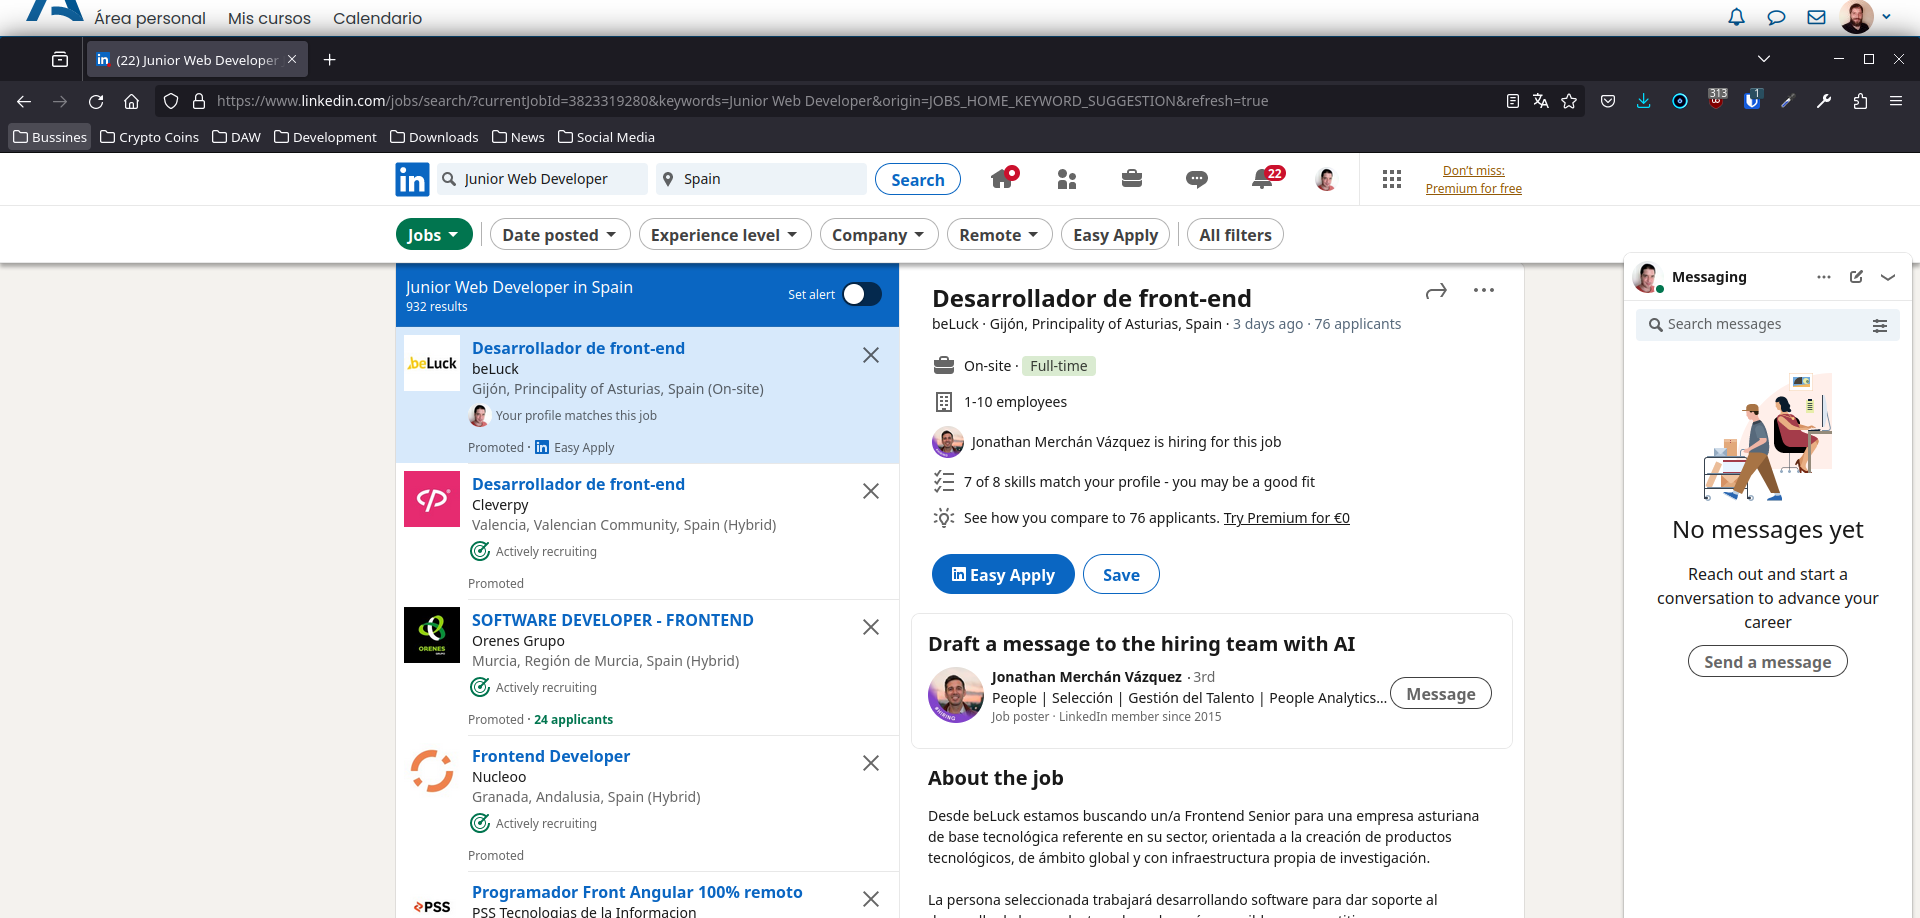
\includegraphics[scale=0.25]{perfil-link-jobs.png}
        \caption{Realizando una búsqueda de empleo}
    \end{figure}

    \item En este último punto, se ha compartido la cuenta de Linkedin en el hilo de la asignatura habilitado para ello, realizándose una captura de la aportación, que se muestra a continuación.

        \begin{figure}[H]
        \centering
        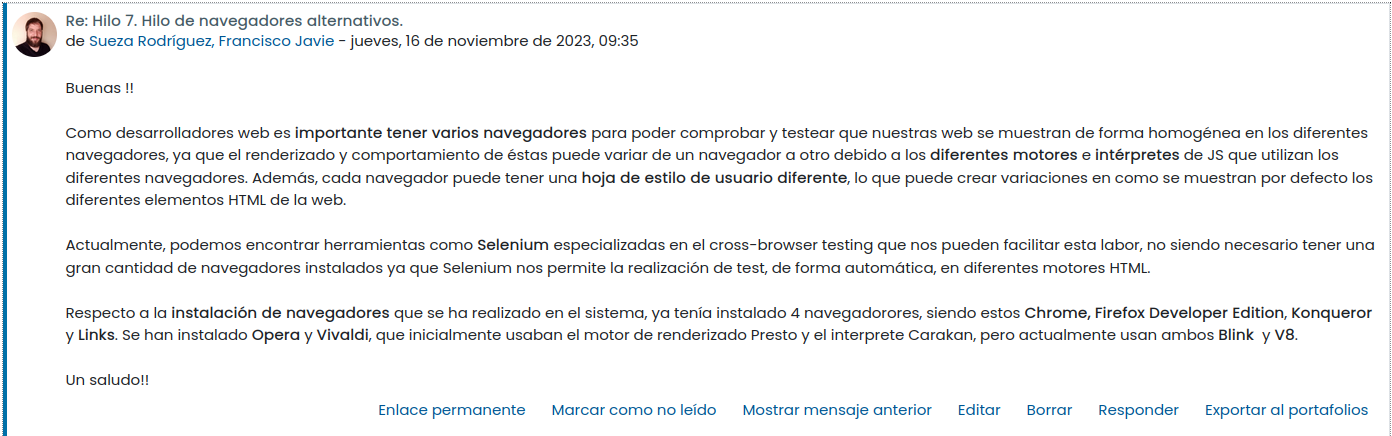
\includegraphics[scale=0.30]{foro-1.png}
        \caption{Contribución al foro con el enlace de LinkedIn}
    \end{figure}

\end{enumerate}

\section{Ejecicio 2: Foro}
\subsection{Enunciado}
Accede al hilo de la unidad 3  "Casos de éxito" y cuenta algún caso de éxito de una empresa o conocido  que hayan tenido éxito a través de las redes sociales. Puedes buscarlo en internet o que sea conocido por ti, incluso igual eres tú mismo!

\subsection{Solución}

En este ejercicio se ha realizado una aportación al foro explicando un caso de éxito en el uso de las RRSS respecto al empleo. No se va a incluir el texto para no duplicar información, ya que podemos verlo integro en la siguiente captura de la intervención en el foro.

Aunque veo que en el foro toda la gente se esta centrando en empresas, yo voy a centrarme en un amigo mío, que se dedica al desarrollo de software y a encontrado prácticamente todos sus puestos de trabajo en LinkedIn.


        \begin{figure}[H]
    \centering
    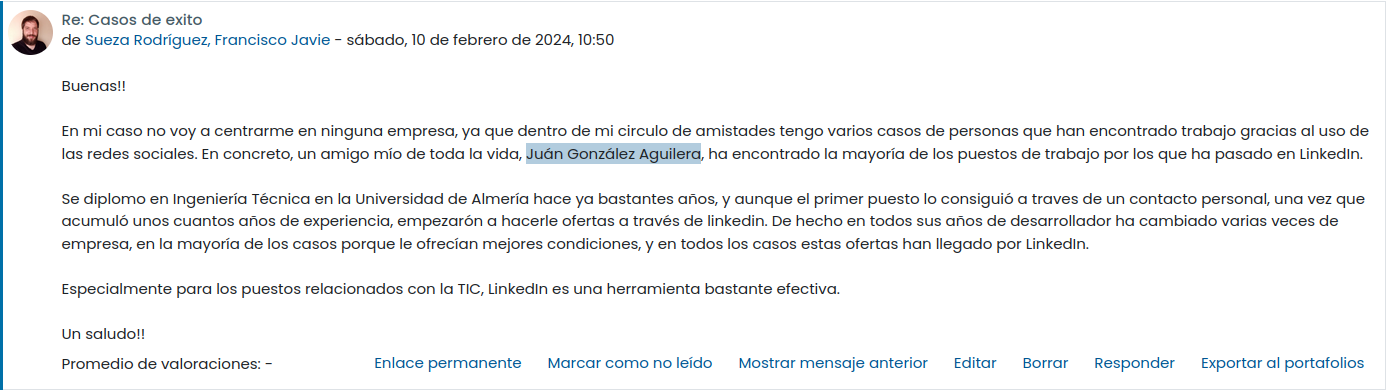
\includegraphics[scale=0.40]{exito.png}
    \caption{Contribución al foro con un caso de éxito}
\end{figure}


% Bibliography

%\newpage
%\bibliography{citas}
%\bibliographystyle{unsrt}

\end{document}